\chapter{Pilotforsøg}\vspace{-.75cm}\label{pilot}
\section{Formål}
Pilotforsøget udføres med henblik på at kunne lave algoritmer ud fra målinger med et accelerometer og gyroskop, som adskiller de tre forskellige aktivitetsformer gang, løb og cykling. Det undersøges derudover hvilke af accelerometerets akser der er essentielle at lave algoritmer ud fra. Ydermere undersøges signalernes frekvens for at undgå aliasing i det endelige system og for at kende nyquistfrekvensen. Sidst undersøges hvilken indflydelse placering af sensoren har på signalets udformning. Dette gøres så det endelige systems signal ikke går i mætning på grund af for stor kraftpåvirkning, og for at undersøge om placering har indflydelse på signalernes udformning.

Til opsamling af data, anvendes en Shimmer 3. Dette er en enhed, som indeholder en række sensorer\fxnote{accelerometer, gyroskop, tryksensor, magnometer, højdemåler}, hvor der til forsøget udelukkende benyttes et accelerometer og et gyroskop. 

%Resultaterne fra pilotforsøget bruges til at designe det endelige system, hvor softwaren for CY8CKIT-043 PSoC 4 M-Series Prototyping Kit skal konfigureres og tilpasses.
Formålet med pilotforsøget er dermed:\vspace{-3mm}
\begin{itemize}
	\item At undersøge hvordan signalerne for gang, løb og cykling adskilles fra hinanden. 
	\item At undersøge hvilken betydning placering af sensorene har for signalets udformning ved de tre aktivitetsformer gang, løb og cykling. 
	\item At bestemme frekvensområdet for signalerne.
	\item At bestemme amplitude for signalerne 
\end{itemize}
%er det nødvendigt at kende signalets frekvensindhold og vide, hvordan forskellige aktivitetsformer påvirker systemet. Målingerne skal undersøges for at kunne lave en algoritme, som kan få sensoren til at skelne imellem de pågældende aktivitetsformer. Derudover skal det bestemmes, hvor sensoren skal placeres på kroppen for mest optimalt udbytte. Derfor er formålet med pilotforsøget følgende:
%\begin{itemize}
%	\item Bestemme hvordan sensoren påvirkes af gang, løb og cykling. (Undersøge signalets udformning for accelerometer og gyroskop ved aktiviteterne; løb, gang og cykling. 
%		- Ligeledes at undersøge placeringen af sensoren ift. påvirkning af signalet.	
%	\item Undersøge hvor mange g-kræfter sensorens målinger ændrer sig alt efter placering på kroppen.
%	\item Undersøge bevægelsesmønstret i signalet i forhold til placering af sensor.
%	\item Bestemme frekvensindholdet for signalet.
%\end{itemize}

\section{Metode}
%Forsøgets metode er bestemt og udført med henblik på at opfylde pilotforsøgets formål. Dette involverer henholdsvis de materialer der skal benyttes samt den fremgangsmåde som ligger til grund for udførelsen.

Til forsøget medtages kun forsøgspersoner, som ikke lider af gener der forhindrer dem i at udføre aktiviteterne gang, løb og cykling. Er en person skadet eller syg, eksluderes denne dermed fra forsøget. Der udføres kun forsøg på gruppemedlemmer, og det er derfor ikke muligt at udføre forsøget på en person fra målgruppen, som er på 8-12 år. Resultaterne kan dermed variere i forhold til målgruppen, da disses vægt og højde vil varierer fra forsøgspersonerne. 

%Forsøget inkluderer udelukkende fuldt funktionsdygtige personer, hvormed ingen forsøgspersoner må have fysiske gener som kan medføre besvær ved udførsel af aktiviterne; gang, løb og cykling. Dermed sikres det, at forsøgets data indeholder normaliserede data som giver grundlag for et validt og repræsentativt datasæt for fysisk funktionsdygtige personer. 

Forsøget vil tage udgangspunkt i tre forudbestemte placeringer på underbenet af enheden, Shimmer3, hvilke kan ses på \figref{fig:sensor_placering}. Disse placeringer er udvalgt på baggrund af \secref{bevaegelse}, hvor det ses at de største bevægelser optræder her i forbindelse med gang, løb og cykling. Accelerometeret registrerer position og acceleration, og det forventes derfor at den største forskel vil kunne ses ved disse placeringer, da det især er distalt for patella, der bevæges under gang og løb. I databehandlingen behandles kun data fra accelerometerets y-akse, da denne på baggrund af \secref{bevaegelse} bør have den største kraftpåvirkning.

%Det er kun placering B der påvirkes af z-aksen ved aktiviteten gang\citep{sabas kilde}, hvormed det formodes at samme påvirkning gælder for løb\citep{RueterboriesSpaichLarsenEtAl2010}. Ud fra bevægelsesanalysen i \secref{bevaegelse}, udledes det ligeledes at alle tre aktiviteter primært er i disse to retninger. 
% Dette vælges på baggrund af bevægelsesanalysen, hvor det blev udledt at den primære bevægelse af  benet ved de tre aktivitetsformer gang, løb og cykling i x- og y-aksens retning \citep{kilde}. \fxnote{måske noget om gyroskop + er det rigtigt i forhold til bevægelsesanalysen??}


% med henhold til æstetiske og brugervenlige aspekter samt \secref{TEORI SENSORER}. \newline
%\textit{Jeg ved ikke helt hvad jeg skal skrive vores begrundelse er ift. det teori om gyroskop, derfor skal de sidste linjer her skrives på senere. Ellers hvis en af jer ved nok om gyroskop til at skrive begrundelsen ;-)}


\subsection{Materialer}
\begin{itemize}
	\item Løbebånd med justerbar hastighed og sikkerhedsbæresele.
	\item Motionscykel.
	\item Shimmer3 sensor med tilhørende holder og strap.
	\item Sportstape.
	\item Computer med følgende software:
	\begin{itemize}
		\item Labview.
		\item Shimmer sensing.
	\end{itemize}
\end{itemize}

\subsection{Fremgangsmåde}
Forsøgets fremgangsmåde er opdelt i to dele. Første del indeholder en opsætning af Shimmer3, mens den anden del er fremgangsmåden for optagelse af data fra forsøget.

\subsubsection{Opsætning af Shimmer3 SUB}
Før forsøgene kan udføres skal Shimmer forbindes korrekt med computeren, og indstilles til at bruge de sensorer der ønskes i pilotforsøget. \vspace{-3mm}
\begin{itemize}
	\item Shimmer forbindes til programmet Labview gennem bluetooth.
	\item Shimmer indeholder en række sensorer, hvoraf følgende skal aktiveres: 
	\begin{itemize}
		\item Widerange Accelerometer.
		\item Gyroscope.
	\end{itemize}
	\item De maksimale arbejdsområder på $\pm$16 g og $\pm$2000 dps vælges, da signalets amplitude endnu er ukendt.
	\item Samplingsfrekvensen indstilles på 512 Hz, da signalets frekvens er ukendt, og denne samplingsfrekvens er den maksimale der kan vælges, når både gyroskopet og accelerometeret er i brug.  
	\item Det er nu muligt at starte stream, og derefter realtime.
\end{itemize}
%Shimmer3 undersøges nu for at kunne konkludere hvorvidt værdierne fra sensorerne er korrekte. Til denne undersøgelse skal akserne for accelerometeret og gyoskopet findes ved opslag i datablad for enheden. Når disse akser er bestemt, benyttes Labview til at optage målinger i. Der startes en ’Stream’ for at undersøge realtime målingerne.
%Først undersøges accelerometerets værdier ved at placere Shimmer3 på en flad, fast overflade. Shimmer3 vendes i 6 forskellige positioner afhængigt af om det er den positive eller negative akse for x, y eller z som undersøges. Værdien for den positive akse for henholdsvis x, y og z skal vise cirka 9,8 m/s, og med negativt fortegn ved den negative akse for x, y og x. I tilfælde af at værdierne er cirka 9,8 m/s, da kan accelerometerets nøjagtighed godtages. Ydermere undersøges gyroskopet ved at spinne Shimmer3 rundt i en række forskellige retninger for at undersøge hvorvidt sensoren reagerer på dette. Hvis gyroskopet registrerer ændringerne, da godtages dennes nøjagtighed. 
%Shimmer3 er forbundet, konfigureret og undersøgt således forsøget efterfølgende kan gennemføres.

\subsubsection{Udførsel af forsøget}
Forsøget udføres på fire forsøgspersoner, som alle skal udføre aktiviteterne gang, løb, hastigheds stigning og cykling. Den nedenstående beskrivelse af forsøgets fremgangsmåde er gældende for én af de forudbestemte placeringer af Shimmer3 på forsøgspersonens højre ben. Alle fire aktiviteter udføres før placeringen ændres, dog benyttes den samme fremgangsmåde til de resterende to placeringer. De tre placeringer kan ses på \figref{fig:sensor_placering}.

\begin{figure}[H]
	\centering
	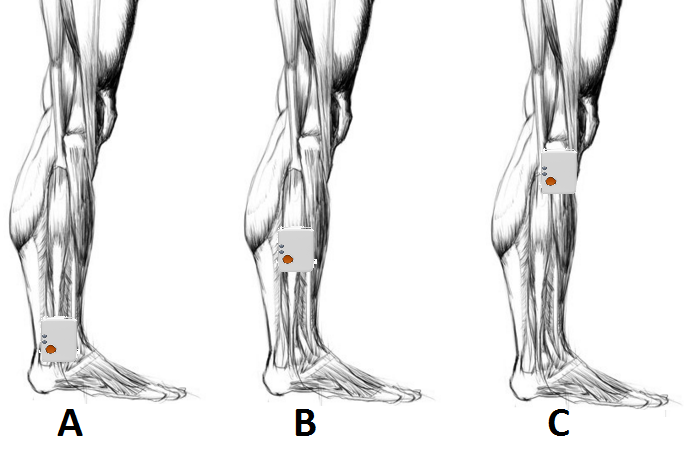
\includegraphics[scale=0.55]{figures/qBilag/Sensor_placering2.png}
	\caption{På figuren ses, hvor sensoren skal placeres under pilotforsøget. Placering A: proximalt for den laterale malleolus. Placering B: medialt på den laterale side af tibia. Placering C: distalt for patella på den laterale side. (Modificeret fra \cite{Perna2016,Shimmer2016})}
	\label{fig:sensor_placering}
\end{figure}

Inden forsøget skal forsøgspersonen fastspændes i en sikkerhedssele, så der ikke opstår skader hvis personen snubler på løbebåndet. Derudover skal forsøgspersonen inden hver måling fortælle hvor på borgskalaen denne befinder sig, og er det under 11 kan målingen påbegyndes. Borgskalaen kan ses på \figref{fig:borgskala}. Denne værdi er valgt for at forsøgspersonen ikke allerede har det som om kroppen er i gang med træning Det sikres dermed at alle forsøgspersoner har samme startbetingelser for alle forsøg. Borgskalaen der benyttes til pilotforsøget kan ses på \figref{fig:borgskala}. 

\begin{figure}[H]
	\centering
	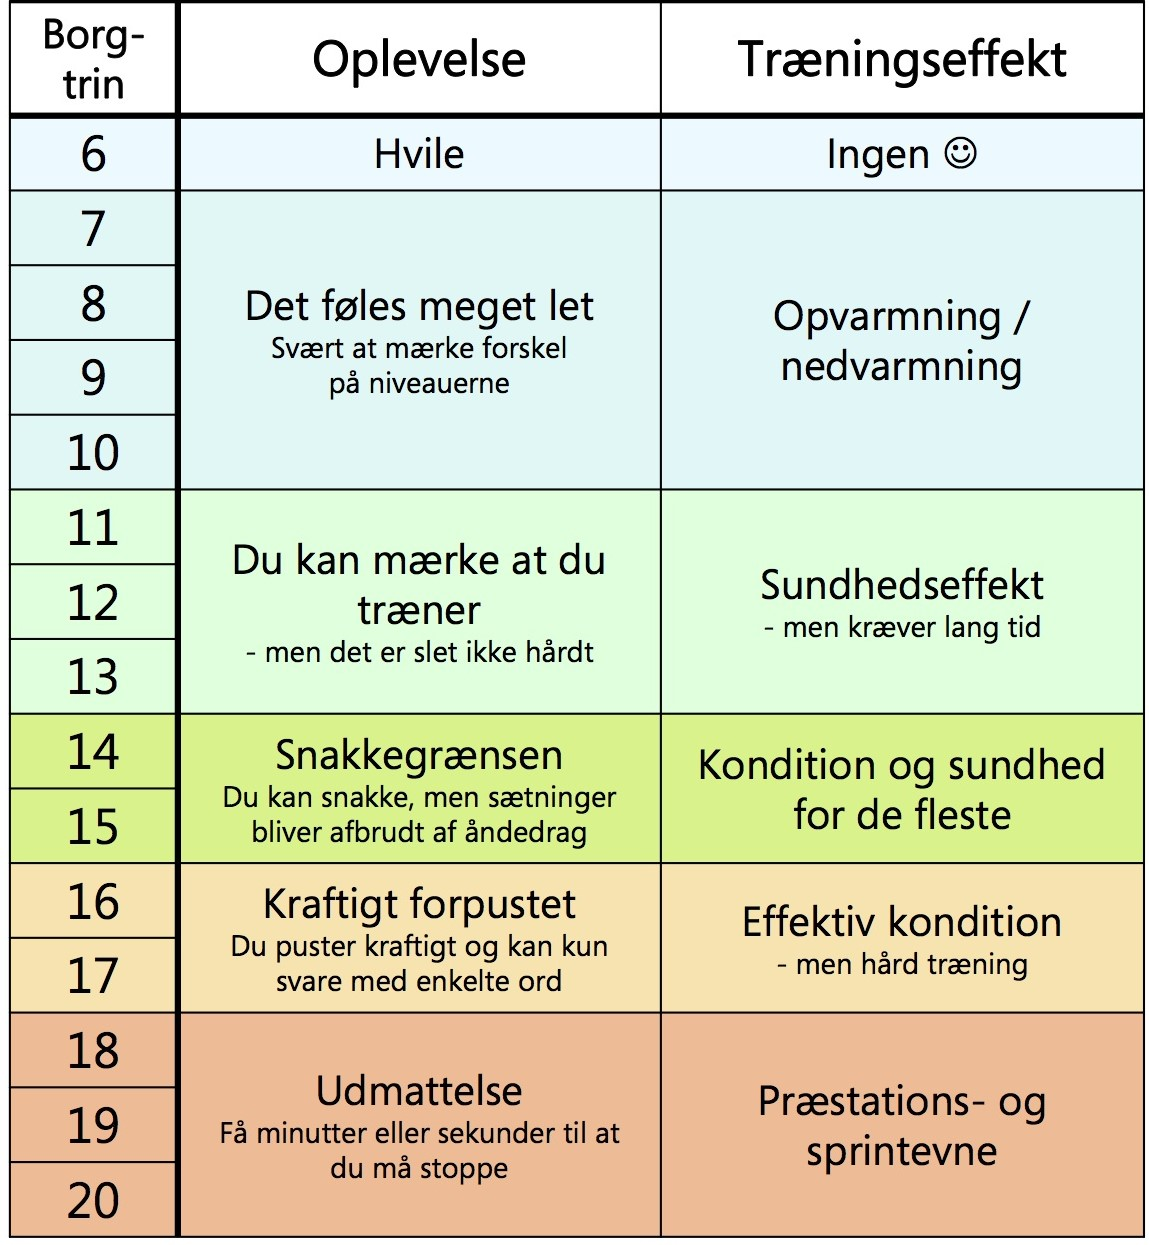
\includegraphics[scale=0.5]{figures/qBilag/Borg-skala.jpg}
	\caption{På figuren ses borgskalaen, som er den der benyttes inden forsøgsstarten. (Modificeret)\cite{Patientinformationen2013})}
	\label{fig:borgskala}
\end{figure}

Første måling er gang, hvor et gangtempo på 4,8 km/t er valgt\citep{Miles2007}. \vspace{-3mm}
\begin{itemize}
	\item Der foretages en baseline på 10 sekunder, hvor forsøgspersonen skal stå oprejst med ret ryg og fødderne placeret parallelt og kigge ligefrem ved baseline målingen.
	\item Løbebåndet indstilles til 4,8 km/t, hvor forsøgspersonen går på løbebåndet indtil en konstant hastighed på løbebåndet opnås. 
	%		\item Forsøgspersonen indikerer når denne føler en homogen bevægelses-cyklus.
	\item Målingen på 45 sekunder igangsættes.
\end{itemize}

Anden måling er løb, et løbetempo på 11,3 km/t er valgt\citep{Miles2007}. \vspace{-3mm}
\begin{itemize}
	\item Der foretages en baseline på 10 sekunder, hvor forsøgspersonen skal stå oprejst med ret ryg og fødderne placeret parallelt og kigge ligefrem ved baseline målingen.
	\item Løbebåndet indstilles til 11,3 km/t, hvor forsøgspersonen løber på løbebåndet indtil en konstant hastighed på løbebåndet opnås. 
	%	\item Forsøgspersonen indikerer når denne føler en homogen bevægelses-cyklus.
	\item Målingen på 45 sekunder igangsættes.
\end{itemize}

Tredje måling foretages på løbebåndet, hvor forsøgspersonen gradvist skal stige i tempo under hele forsøget. Der noteres under forsøget hvornår forsøgspersonen skifter fra gang til løb.  \vspace{-3mm}
\begin{itemize}
	\item Der foretages en baseline på 10 sekunder, hvor forsøgspersonen skal stå oprejst med ret ryg og fødderne placeret parallelt og kigge ligefrem ved baseline målingen.
	\item Målingen igangsættes.
	\item Løbebåndet indstilles til 2 km/t, hvor forsøgspersonen skal gå i 20 sekunder.  
	\item Hastigheden stiger herefter med 2 km/t for hvert 20. sekund, indtil forsøgspersonen har opnået maksimal hastighed, eller løbebåndets maksimale hastighed på 18 km/t. 
	\item Målingen stoppes. 
\end{itemize}

Sidste måling er cykling, hvor et cykeltempo på 20,9 km/t er valgt, hvilket er et højt cykeltempo\citep{Miles2007}. Tempoet er dog underordnet, da der kun ønskes at se på forskellen i selve bevægelsen fra de andre aktivitetsformer, men der er valgt et fast tempo for at få et ensformigt signal. \vspace{-3mm}
\begin{itemize}
	\item Der foretages en baseline på 10 sekunder, hvor forsøgspersonen skal sidde i en naturlig cykelposition på motionscyklen med begge fødder på pedalerne, hvoraf den højre pedal skal være helt i bund. Denne position er valgt, da den er mulig at lave tilnærmelsesvis ens for alle forsøgspersoner, hvormed de får den samme baseline.
	\item Forsøgspersonen træder i pedalerne indtil denne opnår en konstant hastighed på 20,9 km/t ved en belastning på 35 W. Dermed sikres det at alle forsøgspersoner bruger den samme belastning gennem forsøget.  
	\item Målingen på 45 sekunder igangsættes. 
\end{itemize}

Efter de tre placeringer skulle forsøgspersonerne vurdere hvilken placering der var mest behagelig.

\section{Databehandling}
\subsection{Kalibrering af Shimmer}
Forud for pilotforsøgets målinger blev Shimmer kalibreret og testet. For at undersøge hvorvidt kalibreringen af Shimmer fungerede optimalt, blev der opsamlet data til at be-, eller afkræfte dette. Data fra de tre akser, x, y og z blev behandlet. \\
Når Shimmer er placeret i en kalibreringsboks på et bord med henblik på en respektiv akse, bør accelerometeret blive påvirket med $\pm$1 g, mens de resterende akser ikke bør påvirkes.

\begin{figure}[H]
	\centering
	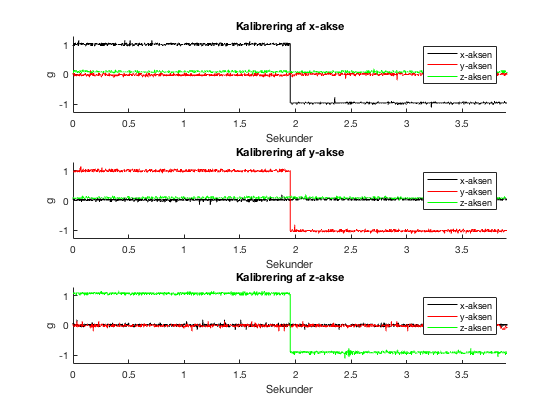
\includegraphics[scale=0.68]{figures/qBilag/kalibreringsdata}
	\caption{På figuren ses kalibreringsdataene tilhørende accelerometerets x, y og z-akse.}
	\label{fig:Ap_Kalibrering}
\end{figure}

For hver akse blev den gennemsnitlige værdi, for henholdsvis den positive- og negative akse, beregnet og sammenholdt med $\pm 1$g. Dermed blev den procentmæssige afvigelse fra tyngdeaccelerationen fundet. Dette resulterede i at x-aksen gennemsnitlig afveg henholdsvis 3,5\% i den negative akse og -2,2\% i den positive akse. Y-aksen afveg gennemsnitligt -2,6\% i den negative akse og -0,6\% i den positive akse. Z-aksen afveg  gennemsnitligt med 8,8\% i den negative akse og 8,0\% i den positive akse. \newline
Kalibreringen blev foretaget for at sikre at et offset ikke var til stede. 

\subsection{Baseline af gang, løb og cykling}
Forud for hver enkelt måling blev der foretaget en baselinemåling som indikation for hvorvidt Shimmer fungerede forud for aktiviteten. Derudover blev det ud fra baseline testet hvorvidt shimmer var i samme position for alle forsøgspersoner ved de forskellige målingers start. Dataene skal afspejle en tilnærmelsesvis fuldstændig tyngdekraftpåvirkning på accelerometerets y-akse, som resultat af Shimmers placering på benet. Baseline blev foretaget for at sikre at shimmer tilnærmelsesvis blev placeret ens på alle forsøgspersoner, hvormed data kunne sammenholdes. 

\begin{table}[H]
	\centering
	\begin{tabular}{cccc}
		\hline
		\rowcolor[HTML]{C0C0C0} 
		{\color[HTML]{333333} Forsøgsperson} & {\color[HTML]{333333} \begin{tabular}[c]{@{}c@{}}Placering A, \\ y-akse {[}g{]}\end{tabular}} & {\color[HTML]{333333} \begin{tabular}[c]{@{}c@{}}Placering B,\\ y-akse {[}g{]}\end{tabular}} & {\color[HTML]{333333} \begin{tabular}[c]{@{}c@{}}Placering C,\\ y-akse {[}g{]}\end{tabular}} \\ \hline
		F1 & 0,98 & 0,99 & 0,97 \\ \hline
		F2 & 1 & 0,99 & 0,96 \\ \hline
		F3 & 0,98 & 0,98 & 0,98 \\ \hline
		F4 & 0,97 & 0,99 & 0,95 \\ \hline
	\end{tabular}
	\caption{I tabellen ses de gennemsnitlige baselineresultater fra accelerometerets y-akse forud for gang.}
	\label{fig:Ap_baselinegang}
\end{table}\vspace{-0.5cm}

\begin{table}[H]
	\centering
	\begin{tabular}{cccc}
		\hline
		\rowcolor[HTML]{C0C0C0} 
		{\color[HTML]{333333} Forsøgsperson} & {\color[HTML]{333333} \begin{tabular}[c]{@{}c@{}}Placering A, \\ y-akse {[}g{]}\end{tabular}} & {\color[HTML]{333333} \begin{tabular}[c]{@{}c@{}}Placering B,\\ y-akse {[}g{]}\end{tabular}} & {\color[HTML]{333333} \begin{tabular}[c]{@{}c@{}}Placering C,\\ y-akse {[}g{]}\end{tabular}} \\ \hline
		F1 & 0,99 & 0,99 & 0,97 \\ \hline
		F2 & 0,99 & 0,99 & 0,96 \\ \hline
		F3 & 0,97 & 0,98 & 0,98 \\ \hline
		F4 & 0,97 & 0,99 & 0,95 \\ \hline
	\end{tabular}
	\caption{I tabellen ses de gennemsnitlige baselineresultater fra accelerometerets y-akse forud for løb.}
	\label{fig:Ap_baselineloeb}
\end{table}\vspace{-0.5cm}

Ved cykling benyttes gyroskopets data, da cykling detekteres som en roterende bevægelse omkring z-aksen. Enheden af dataet heraf er grader per sekund (dps), og dermed bør baselineresultaterne ligge omkring nul.
\begin{table}[H]
	\centering
	\begin{tabular}{cccc}
		\hline
		\rowcolor[HTML]{C0C0C0} 
		{\color[HTML]{333333} Forsøgsperson} & {\color[HTML]{333333} \begin{tabular}[c]{@{}c@{}}Placering A, \\ z-akse {[}dps{]}\end{tabular}} & {\color[HTML]{333333} \begin{tabular}[c]{@{}c@{}}Placering B,\\ z-akse {[}dps{]}\end{tabular}} & {\color[HTML]{333333} \begin{tabular}[c]{@{}c@{}}Placering C,\\ z-akse {[}dps{]}\end{tabular}} \\ \hline
		F1 & -0,98 & -0,83 & -0,87 \\ \hline
		F2 & -0,90 & -0,79 & -0,77 \\ \hline
		F3 & -0,68 & -0,58 & -0,99 \\ \hline
		F4 & -0,89 & -0,92 & -0,85 \\ \hline
	\end{tabular}
	\caption{I tabellen ses de gennemsnitlige baselineresultater fra gyroskopets z-akse forud for cykling.}
	\label{fig:Ap_baselinecykling}
\end{table}\vspace{-0.5cm}

\subsection{Minimum og maksimum g-påvirkning under gang, løb og hastighed}
Dataene fra aktiviteterne, gang, løb og hastigheds stigning blev alle behandlet med henblik på bestemmelse af den maksimale g påvirkning heraf. Dette blev bestemt af den maksimale påvirkning i henholdsvis accelerometerets positive og negative y-akse samt placeringer. Før forsøgene blev baseline målt inden hvert forsøg. 

Den største afvigelse fra tyngdeaccelerationen for gang var på 0.9969\%, hvormed der vurderes at alle baselines har ligget neutralt. \newline
Nedstående tabel viser resultaterne fra gang med et tempo på 4,8 km/t.
\begin{table}[H]
	\centering
	\begin{tabular}{cccc}
		\hline
		\rowcolor[HTML]{C0C0C0} 
		Forsøgsperson & \begin{tabular}[c]{@{}c@{}} Placering A {[}g{]}\end{tabular} & \begin{tabular}[c]{@{}c@{}} Placering B {[}g{]}\end{tabular} & \begin{tabular}[c]{@{}c@{}} Placering C {[}g{]}\end{tabular} \\ \hline
		F1 &  0,09 ; 2,51  & 0,00 ; 2,32  & -2,51 ; 3,33 \\ \hline
		F2 &  -0,19 ; 3,19 & -0,43 ; 3,04 & -0,97 ; 2,84 \\ \hline
		F3 &  -0,24 ; 3,52 & -0,39 ; 3,38 & -0,20 ; 2,51 \\ \hline
		F4 &  -0,04 ; 2,84 & -0,29 ; 3,62 & -0,50 ; 3,52 \\ \hline
	\end{tabular}%
	\caption{I tabellen ses de maksimale positive og negative værdier fra accelerometerets y-akse som resultat af gang med en hastighed på 4,8 km/t. Værdierne er fundet for både placering A, B og C.}
	\label{fig:Ap_maxggang}
\end{table}

Det ses dermed at den maksimale påvirkning i positiv retning af accelerometerts y-akse under gang ved 4,8 km/t var 3,015 Hz $\pm$0,505 for placering A, 3,095 Hz $\pm$0,53 for placering B og 3,05 Hz $\pm$0,47 for placering C.\newline
Den maksimale påvirkning i negativ retning af accelerometerets y-akse under gang ved 4,8 km/t var 0,018 Hz $\pm$0,88 for placering A, -0,28 Hz $\pm$0,28 for placering B og -1,05 Hz $\pm$0,85 for placering C. 

På samme måde blev baseline fundet for løb ved en hastighed på 11,3 km/t, som maksimalt afveg med 0,9930\%. Det vurderes derfor at baseline for alle forsøgspersoner inden løb ligger neutralt. Herefter blev der fundet de maksimale positive og negative værdier for løb, som kan ses i nedstående tabel.  
\begin{table}[H]
	\centering
	\begin{tabular}{cccc}
		\hline
		\rowcolor[HTML]{C0C0C0} 
		Forsøgsperson & \begin{tabular}[c]{@{}c@{}} Placering A {[}g{]}\end{tabular} & \begin{tabular}[c]{@{}c@{}} Placering B {[}g{]}\end{tabular} & \begin{tabular}[c]{@{}c@{}} Placering C {[}g{]}\end{tabular} \\ \hline
		F1 &  -2,03 ; 8,59 & -2,80 ; 5,07 & -4,10 ; 3,33 \\ \hline
		F2 &  -0,97 ; 5,35 & -2,51 ; 6,13 & -4,44 ; 6,52 \\ \hline
		F3 &  -2,12 ; 5,55 & -1,83 ; 5,60 & -2,46 ; 5,60 \\ \hline
		F4 &  -3,48 ; 6,42 & -4,63 ; 6,76 & -3,52 ; 8,30 \\ \hline
	\end{tabular}%
	\caption{I tabellen ses de maksimale positive og negative værdier fra accelerometerets y-akse som resultat af løb med en hastighed på 11,3 km/t. Værdierne er fundet for både placering A, B og C.
	}
	\label{fig:Ap_maxgloeb}
\end{table}
Det ses dermed at den maksimale påvirkning i positiv retning af accelerometerets y-akse under gang ved 11,3 km/t var 6,48 Hz $\pm$2,11 for placering A, 5,89 Hz $\pm$0,87 for placering B og 5,94 Hz $\pm$2,36 for placering C.\newline
Den maksimale påvirkning i negativ retning af accelerometerets y-akse under gang ved 11,3 km/t var -2,15 Hz $\pm$1,18 for placering A, -2,94 Hz $\pm$1,11 for placering B og -3,63 Hz $\pm$1,17 for placering C. 

Slutvis blev accelerometerets y-akse undersøgt ved forsøget hvor forsøgspersonerne gradvist steg i tempo. Baseline for disse målinger afveg med 0,9954\% hvormed det vurderes at baseline for alle målinger var neutrale. Den maksimale påvirkning i henholdsvis positiv og negativ retning der blev detekteret under hastighedsstigningen kan ses i nedstående tabel. 
\textit{Hastigheds stigning:}
\begin{table}[H]
	\centering
	\begin{tabular}{cccc}
		\hline
		\rowcolor[HTML]{C0C0C0} 
		Forsøgsperson & \begin{tabular}[c]{@{}c@{}} Placering A {[}g{]}\end{tabular} & \begin{tabular}[c]{@{}c@{}} Placering B {[}g{]}\end{tabular} & \begin{tabular}[c]{@{}c@{}} Placering C {[}g{]}\end{tabular} \\ \hline
		F1 &  -3,04 ; 8,20  & -4.59 ; 6,28  & -6,66 ; 7,10 \\ \hline
		F2 &  -3,19 ; 10,96 & -4,49 ; 10,48 & -7,58  ; 9,61 \\ \hline
		F3 &  -4,92 ; 10,48 & -4,59 ; 13,13 & -4,63 ; 9,70 \\ \hline
		F4 &  -8,83 ; 16,95 & -7,48 ; 16,32 & -8,01 ; 15,35 \\ \hline
	\end{tabular}%
	\caption{I tabellen ses de maksimale positive og negative værdier fra accelerometerets y-akse som resultat af hastigheds stigning. Værdierne er fundet for både placering A, B og C.}
	\label{fig:Ap_maxghastighed}
\end{table}
Det ses dermed at den maksimale værdi målt i påsitiv etning på accelerometerets y-akse under hastighedsstigningen var 11,65 Hz $\pm$5,3 ved placering A, 11,55 Hz $\pm$4,77 for placering B og 10,44 Hz $\pm$4,91 for placerinng C. \newline
Den maksimale påvirkning i negativ retning for accelerometerets y-akse under hastighedsstigningen var -5,00 Hz $\pm$1,96 for placering A, -5,29 Hz $\pm$0,8 for placering B og -6,72 Hz $\pm$2,09 for placering C.

\subsection{Maksimal omdrejninger per sekund under cykling}
Dataene fra aktiviteten, cykling, blev behandlet med henblik på bestemmelse af den maksimale amplitude fra gyroskopet. Dette blev bestemt ved at beregne den maksimale peak-to-peak, under udførelsen af cykling. Dataene blev kun behandlet med henblik på gyroskopets z-akse, som resultat af \secref{bevaegelse}. Inden dataopsamling for cykling, blev der målt en baseline. Den maksimale afvigelse fra nul var -0,9979\%, hvormed det vurderes at alle målinger havde en neutral baseline. Dataene fra forsøget kan ses i nedstående tabel.

\begin{table}[H]
	\centering
		\begin{tabular}{cccc}
			\hline
			\rowcolor[HTML]{C0C0C0} 
			Forsøgsperson & \begin{tabular}[c]{@{}c@{}} Placering A {[}g{]}\end{tabular} & \begin{tabular}[c]{@{}c@{}} Placering B {[}g{]}\end{tabular} & \begin{tabular}[c]{@{}c@{}} Placering C {[}g{]}\end{tabular} \\ \hline
			F1 & -148,23 ; 108,29   & -209,82 ; 118,60   & -188,66 ; 98,29  \\ \hline
			F2 & -108,42 ; 108,11   & -133,11 ; 114,94	 & -150,43 ; 120,61 \\ \hline
			F3 & -208,29 ; 136,28  	& -196,95 ; 140,18	 & -195,43 ; 151,10 \\ \hline
			F4 & -182,56 ; 152,13  	& -159,82 ; 138,35	 & -152,62 ; 136,83 \\ \hline
		\end{tabular}%
	\caption{I tabellen ses de maksimale positive og negative værdier fra gyroskopets z-akse som resultat af cykling med en hastighed på 20,9 km/t. Værdierne er fundet for både placering A, B og C.}
	\label{fig:Ap_maxghastighed}
\end{table}
Det ses dermed at den maksimale påvirkning i positiv retning af gyroskopet under cykling ved en hastighed på 20,9 km/t var 126,20 dps $\pm$25,93 for placering A, 128,02 dps $\pm$12,16 for placering B og 126,71 dps $\pm$24,39 for placering C. 
Den maksimale påvirkning i negativ retning er -161,88 dps $\pm$53,46 for placering A, -174,93 dps $\pm$41,82 for placering B og -171,79 dps $\pm$21,36 for placering C. 

\subsection{Afgrænsning af placering}
Databehandling vil ud fra de maksimale værdier tage udgangspunkt i placering A. Dette gøres på baggrund af at denne er den mest optimale placering i forhold til komfort for brugeren, da tre ud af fire forsøgspersoner foretrak denne placering. Den maksimale værdi for placering A overskrider den maksimale accelerationskraftpåvirkning med 0,95 g. Det vurderes dog at placering A vil være optimal at bruge da de 16,95 g repræsenteres i form af hælnedslag. Det vil stadig være muligt at adskille hælnedslag fra tåafsæt selvom det vil klippes ved 16 g. \newline
Gyroskopets data viser ligeledes at det er muligt at benytte placering A, da denne viser at cykling ikke resulterer i en høj dps. 
På baggrund af dette vil der i det resterende databehandling tages udgangspunkt i placering A, som kan ses i to sekunders interval for hver af de fire forsøgspersoner på \figref{raa_data}.

\begin{figure}[H]
	\centering
	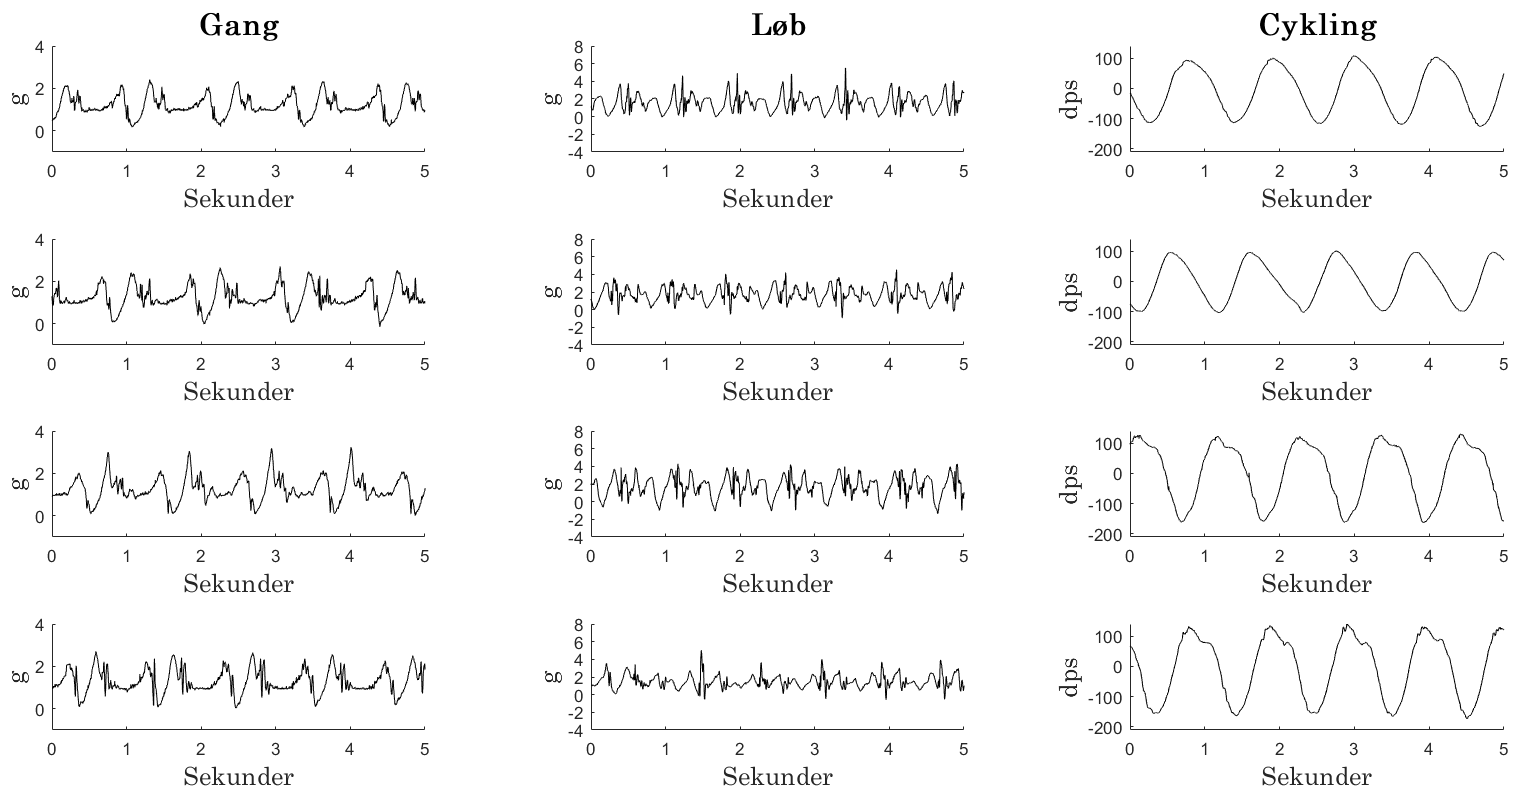
\includegraphics[scale=0.38]{figures/qBilag/raa_data}
	\caption{På figuren ses det ubehandlede data fra de tre aktivitetstyper gang, løb og cykling optaget på henoldsvis et accelerometer og et gyroskop ved placering A.}
	\label{raa_data}
\end{figure}


\subsection{Frekvensindhold af gang, løb og cykling}
Dataene fra aktiviteterne, gang og løb blev behandlet for at bestemme signalernes frekvensindhold. Resultatet af dette muliggør bestemmelsen af samplingsfrekvensen vedrørende accelerometeret og gyroskopet. Der blev foretaget en frekvensdomæne analyse, hvilket muliggør visualisering af signalets magnitude ved forskellige frekvenser, hvoraf energien af signalet kommer til udtryk.

\begin{figure}[H]
	\centering
	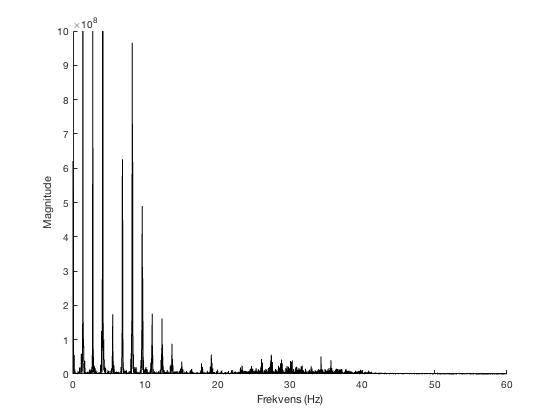
\includegraphics[scale=0.68]{figures/qBilag/fft_f1_loeb}
	\caption{På figuren ses frekvensdomænet af aktiviteten løb for forsøgsperson 1. Den fuldstændige magnitude for de lave frekvenser vises ikke til fulde. Hvis dette skulle være tilfældet ville de mindste magnituder på figuren blive udskalleret.}
	\label{fig:Ap_FFt}
\end{figure}
Frekvensdomæneanalysen vises kun for løb af F1 da frekvensspektrummet var størst heraf. Derudover vises den ikke for gang, da denne ydermere var lavere end for løb, og da begge aktiviteter skal detekteres med et accelerometer, skal de have samme samplingsfrekvens. Dermed vises kun frekvensspektrummet or løb, da systemets samplingsfrekvens bestemmes i forhold til den højest målte frekvens.

Dataene fra aktiviteten, cykling blev behandlet for at bestemme signalernes frekvensindhold, med henblik på bestemmelsen af samplingsfrekvensen vedrørende gyroskopet.
\begin{figure}[H]
	\centering
	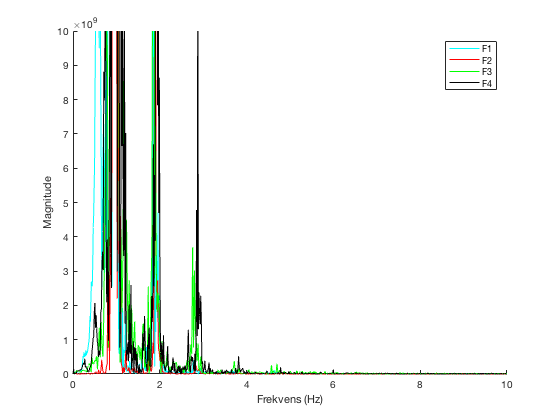
\includegraphics[scale=0.68]{figures/qBilag/cykling_frekvens}
	\caption{På figuren ses frekvensdomænet af aktiviteten cykling for alle forsøgspersoner. Den fuldstændige magnitude for de lave frekvenser vises ikke til fulde. Hvis dette skulle være tilfældet ville de mindste magnituder på figuren blive udskalleret.}
	\label{fig:Ap_cyklingfrekvens}
\end{figure}

\subsection{Accelerometer karakteristika vedrørende gang og løb}
Dataene fra aktiviteten gang og løb blev behandlet med henblik på bestemmelse af signalets karakteristika, således en sammenligning og senere algoritmedesign blev muliggjort. Dataene fra accelerometerets y-akse blev for alle forsøgspersoner lavpas filtreret ved 45 Hz, grundet frekvensspektret på \figref{fig:Ap_FFt}. Derudover vlev signalet differentieret hvormed områderne med størst hældningskoefficient kommer til udtryk. Dermed fremhæves hælnedslag og tåafsæt da disse events har en stor hældning.
\newpage
\textit{Gang:}
\begin{figure}[H]
	\centering
	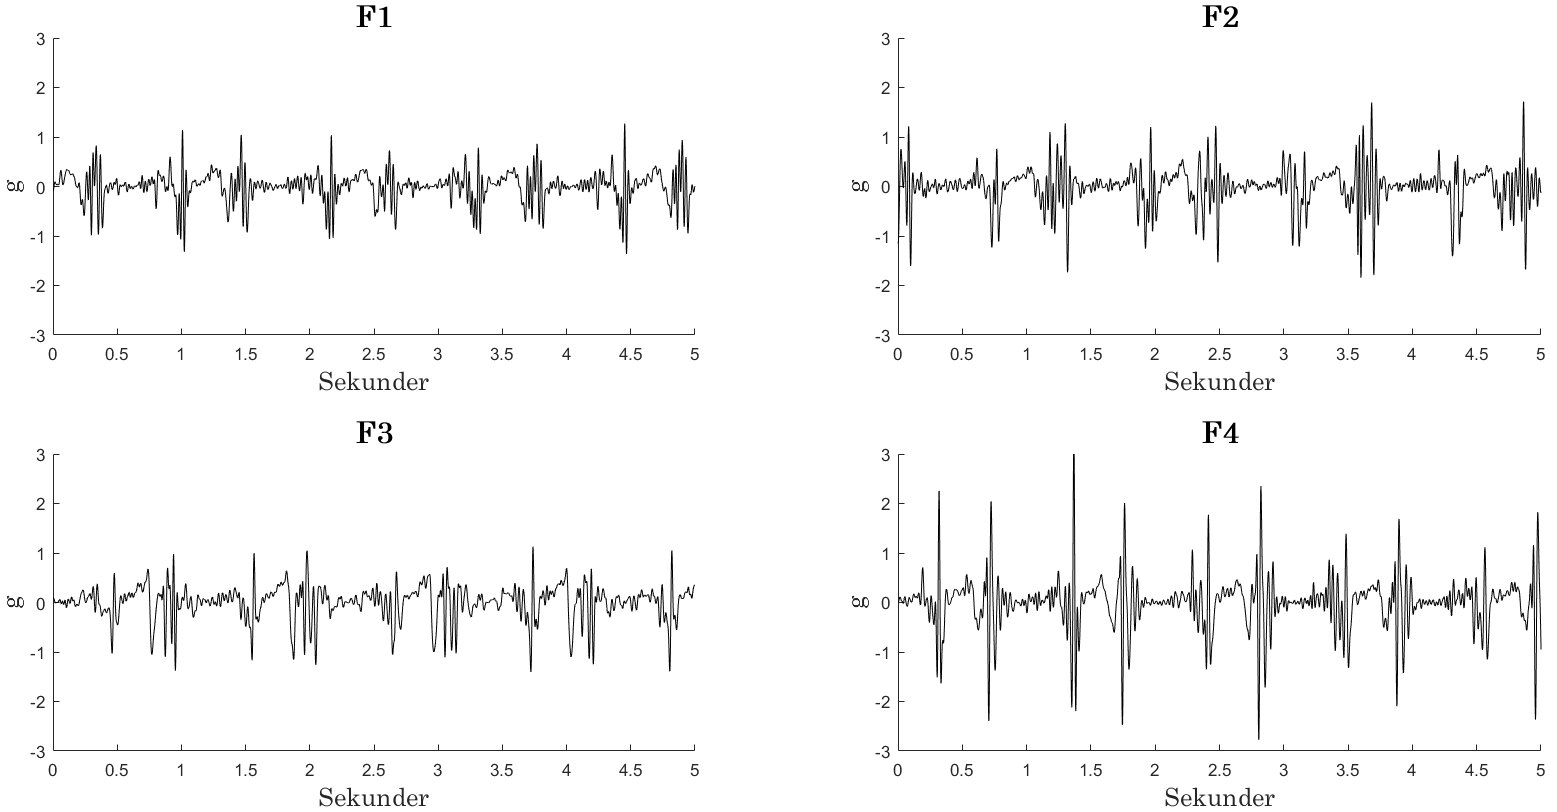
\includegraphics[scale=0.6]{figures/qBilag/gang_diff}
	\caption{På figuren ses det filtrerede og differentierede data fra aktiviteten gang for alle forsøgspersoner.}
	\label{fig:Ap_gangdiff}
\end{figure}

Det ses at hælnedslagg og tåafsæt fremgår tydligere end på \figref{raa_data} for både gang, som kan ses på \figref{fig:Ap_gangdiff} og løb, som kan ses på \figref{fig:Ap_loebdiff}.

\begin{figure}[H]
	\centering
	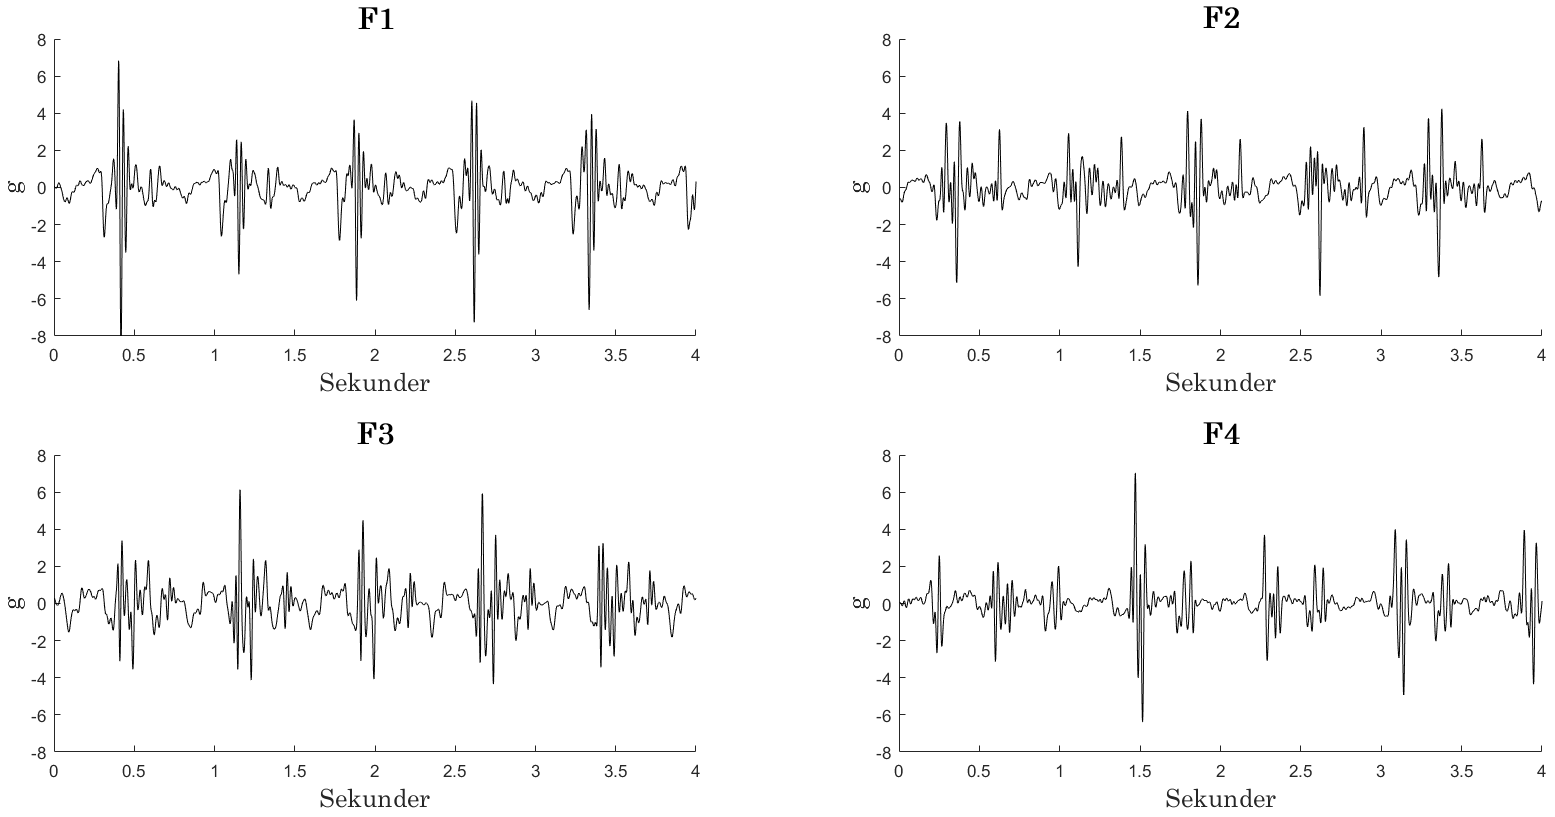
\includegraphics[scale=0.6]{figures/qBilag/loeb_diff}
	\caption{På figuren ses det filtrerede differentierede data fra aktiviteten løb for alle forsøgspersoner.}
	\label{fig:Ap_loebdiff}
\end{figure}

\subsection{Gyroskop karakteristika vedrørende gang, løb og cykling}
Dataene fra aktiviteterne gang, løb og cykling, blev behandlet med henblik på bestemmelse af signalets karakteristika. Dette blev udført ved at sammensætte forsøgspersonernes data, således en sammenligning blev muliggjort. Aktiviteterne gang og løb blev behandlet for at sikre dette ikke havde samme karakteristika som cykling, med henblik på algoritmedesign. Dataene blev kun behandlet med henblik på gyroskopets z-akse, som resultat af \secref{bevaegelse}.  

\textit{Gang:}
\begin{figure}[H]
	\centering
	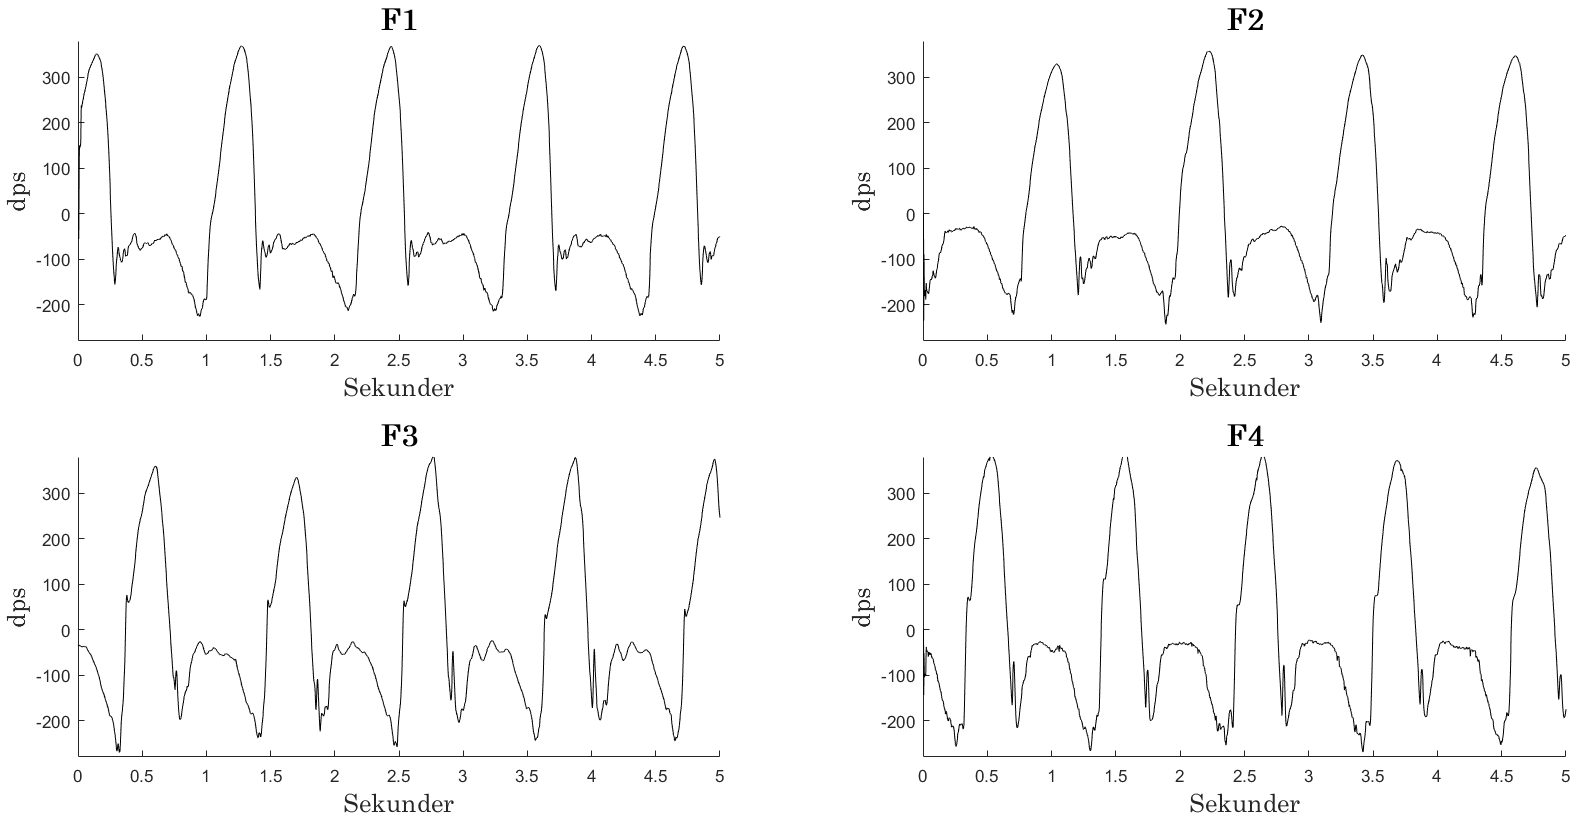
\includegraphics[scale=0.5]{figures/qBilag/gang_gyro}
	\caption{På figuren ses dataene fra gang ved 4,8 km/t fra de fire forsøgspersoner. Dataene er fra gyroskopets z-akse.}
	\label{fig:Ap_cykling}
\end{figure}

\textit{Løb:}
\begin{figure}[H]
	\centering
	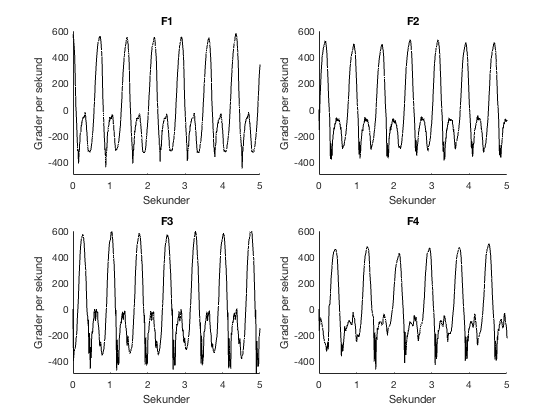
\includegraphics[scale=0.5]{figures/qBilag/loeb_gyro}
	\caption{På figuren ses dataene fra løb ved 11,3 km/t fra de fire forsøgspersoner. Dataene er fra gyroskopets z-akse.}
	\label{fig:Ap_cykling}
\end{figure}

\textit{Cykling:}
\begin{figure}[H]
	\centering
	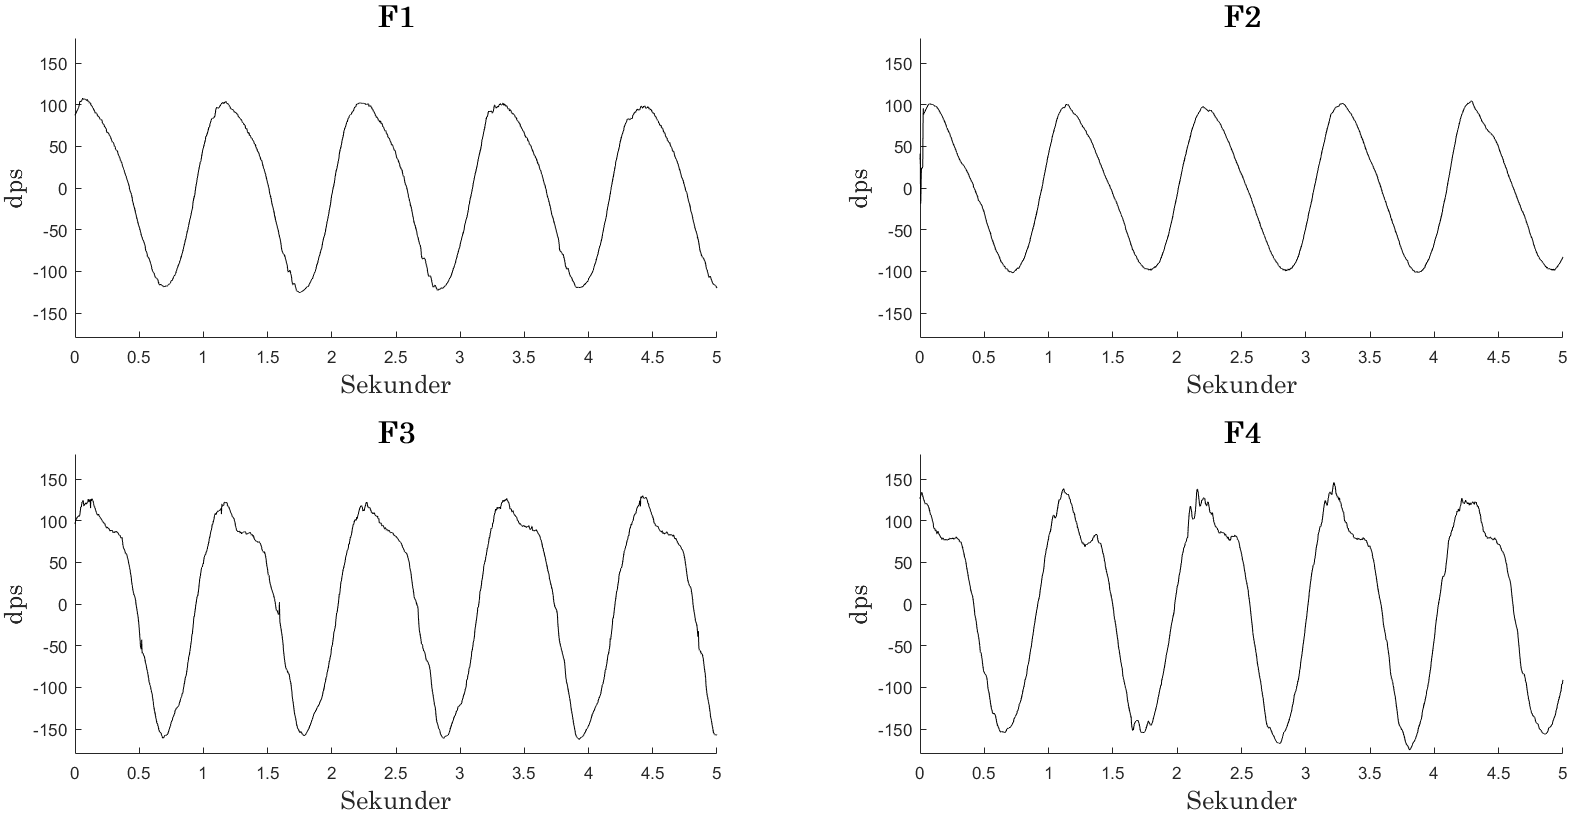
\includegraphics[scale=0.5]{figures/qBilag/cykling_gyro}
	\caption{På figuren ses dataene fra cykling ved 20,9 km/t fra de fire forsøgspersoner. Dataene er fra gyroskopets z-akse.}
	\label{fig:Ap_cykling}
\end{figure}

\section{Diskussion}
\subsection{Kalibrering af Shimmer}
Resultatet af databehandlingen bevirker at kalibreringen af Shimmer antages at være tilstrækkelig. Dette antages at være tilstrækkeligt, da y-aksen  afviger med henholdsvis -2,6\% i den negative akse og -0,6\% i den positive akse, fra den teoretiske værdi. En eventuel fejlkilde til at denne fejlmargin forekom, kunne være at bordet hvorpå Shimmer var placeret, ikke var i vatter.

\subsection{Baseline af gang, løb og cykling}
Baselinemålingerne for henholdsvis gang og løb resulterede i en enslignende påvirkning. Som forventet var g påvirkningen ikke 1 g, hvilket kan være et resultat af at Shimmer ikke er placeret ortogonalt på y-aksen på benet. I og med Shimmer ikke var placeret ortogonalt på benet, kan der være opstået en lille hældning, hvorfor y-aksen ikke påvirkes med præcist 1 g. Resultaterne fra disse målinger indikerer at Shimmer har optaget data som stemmer overens med antagelsen om den tilnærmelsesvise påvirkning på 1 g. 

Resultaterne fra baselinemålingerne vedrørende cykling ligger som forventet omkring nul, hvilket er et resultat af at Shimmer ikke er blevet påvirket i z-aksen i nogen væsentlig grad, da benet ikke bevæges. Resultaterne af disse målinger indikerer at Shimmer har optaget data som stemmer overens med antagelsen om den tilnærmelsesvise påvirkning på 0 dps\fxnote{maksimal afvigelse på -0,9979}. 

\subsection{Maksimal g-påvirkning under gang, løb og hastighed} \label{app:maxg}
Resultatet af databehandlingen vedrørende de tre aktiviteter med henblik på bestemmelsen af den maksimale g påvirkning, medførte at aktiviteten med hastighedsstigning havde den største påvirkning. Resultaterne fra placering A, B eller C fra F1, F2 og F3 ikke overskrider $\pm 16g$. Resultaterne fra F4 overskrider 16 g med 0,95 g. Dette vuredres dog til ikke at have en væsentligt betydning, hvoraf den mest fordelagtige placering vælges. Med baggrund i \secref{succeskrav} og \secref{funktionellekrav} skal placeringen ikke være til gene for barnet, og så skal nemt af-, og påmonteres, hvoraf placering A er valgt, da denne blev valgt som den mest komfortable bland forsøgspersonerne. Dette medfører at den videre resultatbehandling udelukkende tog udgangspunkt i placering A. 

\subsection{Maksimal omdrejninger per sekund under cykling}
Resultatet af databehandlingen vedrørende maksimal omdrejninger ved cykling resulterede i et spænd mellem 216,5 dps og 320,4 dps. Dette kan være et resultat af at forsøgspersonerne ikke har holdt samme hastighed, hvoraf en pludselig acceleration kan betyde en ændring som ikke er relateret til cykling ved 20,9 km/t. I takt med at der maksimalt blev registreret 320,4 dps, er dette medbestemmende vedrørende valg af et endeligt gyroskop. Et gyroskop til det endelige system skal heraf have et arbejdsområde som er større end 320,4 dps, men det præcise arbejdsområde vides ikke, da en hastighedsstigning ikke blev foretaget for cykling.

\subsection{Frekvens indhold af løb og cykling}
Databehandlingen af frekvensindholdet fra gang og løb medførte at det største frekvensspektrum lå mellem 0 og 45Hz. Dette medfører at samplingsfrekvensen vedrørende data fra accelerometeret kan bestemmes. 

Databehandling af frekvensindholdet fra cykling medførte at det største frekvensspektrum lå mellem 0 og 6 Hz. Dette medfører at samplingsfrekvensen vedrørende data fra gyroskopets kan bestemmes. 

\subsection{Accelerometer karakteristika vedrørende gang og løb}
Databehandlingen vedrørende accelerometerets karakteristika af gang og løb resulterede i en sammenligning af dataene. Dataene fra gang viser to events hvor peaks fremstår. Disse har en relativ kort afstand til hinanden, efterfulgt af en længere pause, hvilket flere figurer i \secref{bevaegelse} viser som henholdsvis hælnedslag og tåafsæt. Ligeledes for løb var disse forskellige events, som også antages værende hælnedslag og tåafsæt. Der forekom dog yderligere et harmonisk peak som var betydeligt større end de andre events. Yderligere behandling af aktiviteternes data med anerkendte algoritmer kan være nødvendig, men databehandlingen medførte at gang og løbs karakteristika kan bestemmes og heraf adskilles. Dette er muligt idet varigheden mellem de antagede hælnedslag forekommer $\approx$~0,43 sekunder hurtigere ved løb end ved gang.\fxnote{hvis dette skal med skal er overvejes om man altid kan sige 0,43 sekunder, eller om man skal lave det relativt i forhold til tid (60/40)}

\subsection{Gyroskop karakteristika vedrørende gang, løb og cykling}
Databehandlingen af gyroskopets karakteristika vedrørende gang, løb og cykling resulterede i en sammenligning heraf. Resultatet af dette tyder på, at data fra et gyroskops z-akse tilhørende cykling, tilnærmelsesvis kan afspejles som en sinus-bølge, samt at gang og løb antageligvis ikke kan forveksles heraf. Dette muliggør algoritmedesign med henblik på detektering af cykling. Det kan antages at resultater fra cykling ved forskellige hastigheder vil påvirke signalet i en grad hvor frekvens og amplitude ændres.

\section{Konklusion}
I pilotforsøget blev aktiviteterne gang, løb og cykling undersøgt i en biomekanisk sammenhæng. Ud fra kalibreringen vurderes shimmer til at måle korrekt i de forskellige akser. Derudover vise alle baselines at blive påvirket med mindre end 1\% vigende fra det forventede, hvormed det vurderes at alle data kan sammenlignes, da shimmer tilnærmelsesvis er placeret ens ved alle målinger for alle forsøgspersoner. \newline
Signalerne for gang og løb adskilles ved at de maksimale målte amplituder for løb tilnærmelsesvis er dobbelt så stor, som for gang, men ellers ser signalerne ensformige ud. Cykling målt med et gyroskop adskilles væsentligt fra gang og løb, da cykling ikke har store peaks, men i stedet er formet som en sinuslignende kurve. \newline
Signalernes udformning i forhold til placering har ikke en indflydelse på amplituden for gang. For løb stiger den positive amplitude imidlertid jo mere distalt sensoren placeres, mens den stiger i negativ amplitude jo mere proximalt sensoren placeres. Hastighedsstigningen påvirkes på samme måde af placeringen som løb, mens amplituden ved cykling stort set ikke påvirkes efter placeringen. \newline
Frekvensspektrummet for gang og løb vælges ud for de laveste og højeste målte frekvenser, hvormed et frekvensspektrum på 0-45 Hz bestemmes. Frekvensspektrummet for cykling ligger på 0-6 Hz.\newline
Ud fra pilotforsøget vælges placering A som den mest optimale, da data ikke overskrider 16 g i en grad der vil ødelægge signalet, og denne placering er den mest optimale i forhold til komfort. Derudover vælges et accelerometer med minimum 16 g og et gyroskop med minimum 320 dps, hvor gyroskopet også skal have mulighed for at være i deep sleep. 



